\section{Quantum Capacity of Quantum Channels}

\begin{frame}{Quantum Capacity of a Quantum Channel}
The quantity capacity $Q(\mathcal{N})$ of a quantum channel is defined as follows (where $\ket{\psi} = U^{\mathcal{N}}_{A' \rightarrow BE} \ket{\phi}_{AA'}$).
\begin{tcolorbox}
\begin{align*}
Q(\mathcal{N}) &= \max_{\phi_{AA'}} \left[ S(B)_\rho - S(AB)_\rho \right] \\
&= \max_{\phi_{AA'}} \left[ S(B)_\psi - S(E)_\psi \right]
\end{align*}
\end{tcolorbox}

\begin{figure}
    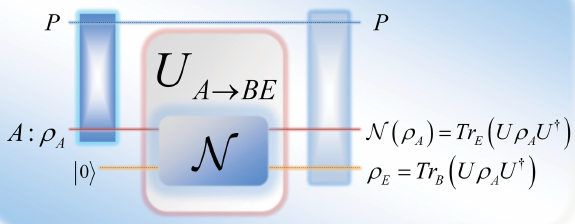
\includegraphics[width=0.5\textwidth]{figures/quantum_communication_quantum_channel.png}
    \caption{Quantum communication through a quantum channel \cite{Gyongyosi_2018}.}
\end{figure}
\end{frame}

\begin{frame}{Properties: Quantum Capacity of a Quantum Channel}
\begin{itemize}
    \setlength{\itemsep}{1.5em}
    \item Non-negativity
    $$Q(\mathcal{N}) \geq 0$$
    \item Non-additivity
    $$Q(\mathcal{N} \otimes \mathcal{M}) \neq Q(\mathcal{N}) + Q(\mathcal{M})$$
    \item Relation with other capacities
    $$Q(\mathcal{N}) \leq P(\mathcal{N}) \leq C(\mathcal{N})$$
\end{itemize}
\end{frame}

\begin{frame}{Proof: Relation with other capacities}
We will consider a pure state that maximizes the quantum capacity. Let $\sigma_{XA'}$ denote the augmented classical-quantum state that correlates with index $x$.
$$\sigma_{XA'} = \sum_{x} p_X(x) \ket{x}\bra{x} \otimes \ket{\phi_x}\bra{\phi_x}_{A'}$$

\begin{align*}
Q(\mathcal{N}) &= \max_{\rho} \left[ S(B)_{\rho} - S(E)_{\rho} \right] \\
&= S(B)_{\sigma} - S(E)_{\sigma}\\
&= S(B)_{\sigma} - S(B|X)_{\sigma} - S(E)_{\sigma} + S(B|X)_{\sigma}\\
&= I(X;B)_{\sigma} - I(X;E)_{\sigma} \\
&\leq \max_{\rho} \left[ I(X;B)_{\rho} - I(X;E)_{\rho} \right] \\
&\leq P(\mathcal{N})
\end{align*}
\end{frame}
